\section{Abstraction: Networked conversations}

\begin{table}
	\resizebox{\linewidth}{!}{
		\begin{tabular}{l|p{8cm}}
			\textbf{Terminology} & \textbf{stands for}\\
			$RP$   & Root post which begins a new thread on a subreddit \\
			$OP$  & Original poster who posts the Root post for a thread \\
			$BP$   & A Poster who has at-least one symmetric response from the $OP$ after his comment\\
			$AP$   & Asymmetric poster who responds to $OP$ but never gets a response back \\
			$SW$ & The suicide watch Subreddit \\
			$FP$  & Front page of Reddit. \\
			$TD$ & The Donald Subreddit \\
			$AS$ & AskScience subreddit \\
	\end{tabular}}
	\caption{Notations and Terms.}\label{notations}
\end{table}


\label{Sec:Conversations}
To understand the dynamics of supportive conversations, we first need to formalize the abstraction of networked conversations. In case of forum based platforms where users interact in a nested dialogue fashion, and original poster or $OP$ posts a start of a thread. This thread is then open for comments by all the community users. In case of Reddit, such a community is called a Subreddit, which is a moderated collection of users who subscribe to it. These users may post new threads onto the subreddit as far as the post follows the subreddit rules. Enforcement of these rules is the responsibility of the moderators. 

The user who starts a thread is called the Original Poster or $OP$ and the headlining post which the $OP$ begins with is called the Root Post or $RP$. We represent the data using two abstractions. One abstraction is called the \textbf{User Graphs} abstraction. In this method, we represent each thread as a directed graph $G\{V,E,W\}$ where $V$ is the set of all users participating in a particular thread and $E$ are the directed  edges which correspond to interactions between two users $V_i , V_j  \in V$. The weight of each directed edge $E_{ij}$ corresponds to the average Jaccard coefficient calculated on topics covered by posts done by $V_i$ to user $V_J$. 
Formally if $T_i$ is the content of the post posted by $V_i$ and $T_j$ is the content of the post posted by $V_j$ and if $F$ is a topic model trained on the corpus of all texts such that $F(T) \mapsto [t_0 , t_1 \ldots t_n ]$ where $t_k$ is the topic that is present in text $T$, then 
\begin{equation}
	W_{ij} = \frac{F(T_i) \cap F(T_j)}{F(T_i) \cup F(T_j)}
\end{equation}
Where $W_{ij}$ is the edge weight between node $V_i$ and node $V_j$.

The Second abstraction to work with in this paper is the \textbf{Reply Graph} abstraction. We formulate a reply graph $R\{P,E\}$ as a thread of multi-layered posts in a thread in response to the root post $RP$ in the sub-reddit. Each graph $R$ consists of posts $P_i , P_j , i,j \in N$ , where N+1 is the total number of responses in the thread and Edges $E_{ij}$such that and Edge $E_{ij}$ exists $iff$ post $P_i$ was in response to post $P_j$ in the hierarchy of responses. This abstraction works well in modelling the conversational nature of these forums.  For convienece of the reader, we present a couple of example pairs from SW and TheDonald subreddit in Figure \ref{Fig:GraphExamples}
\begin{figure*}[!ht]
	\centering
	% \hspace*{-5mm}
	\subfloat[]{
		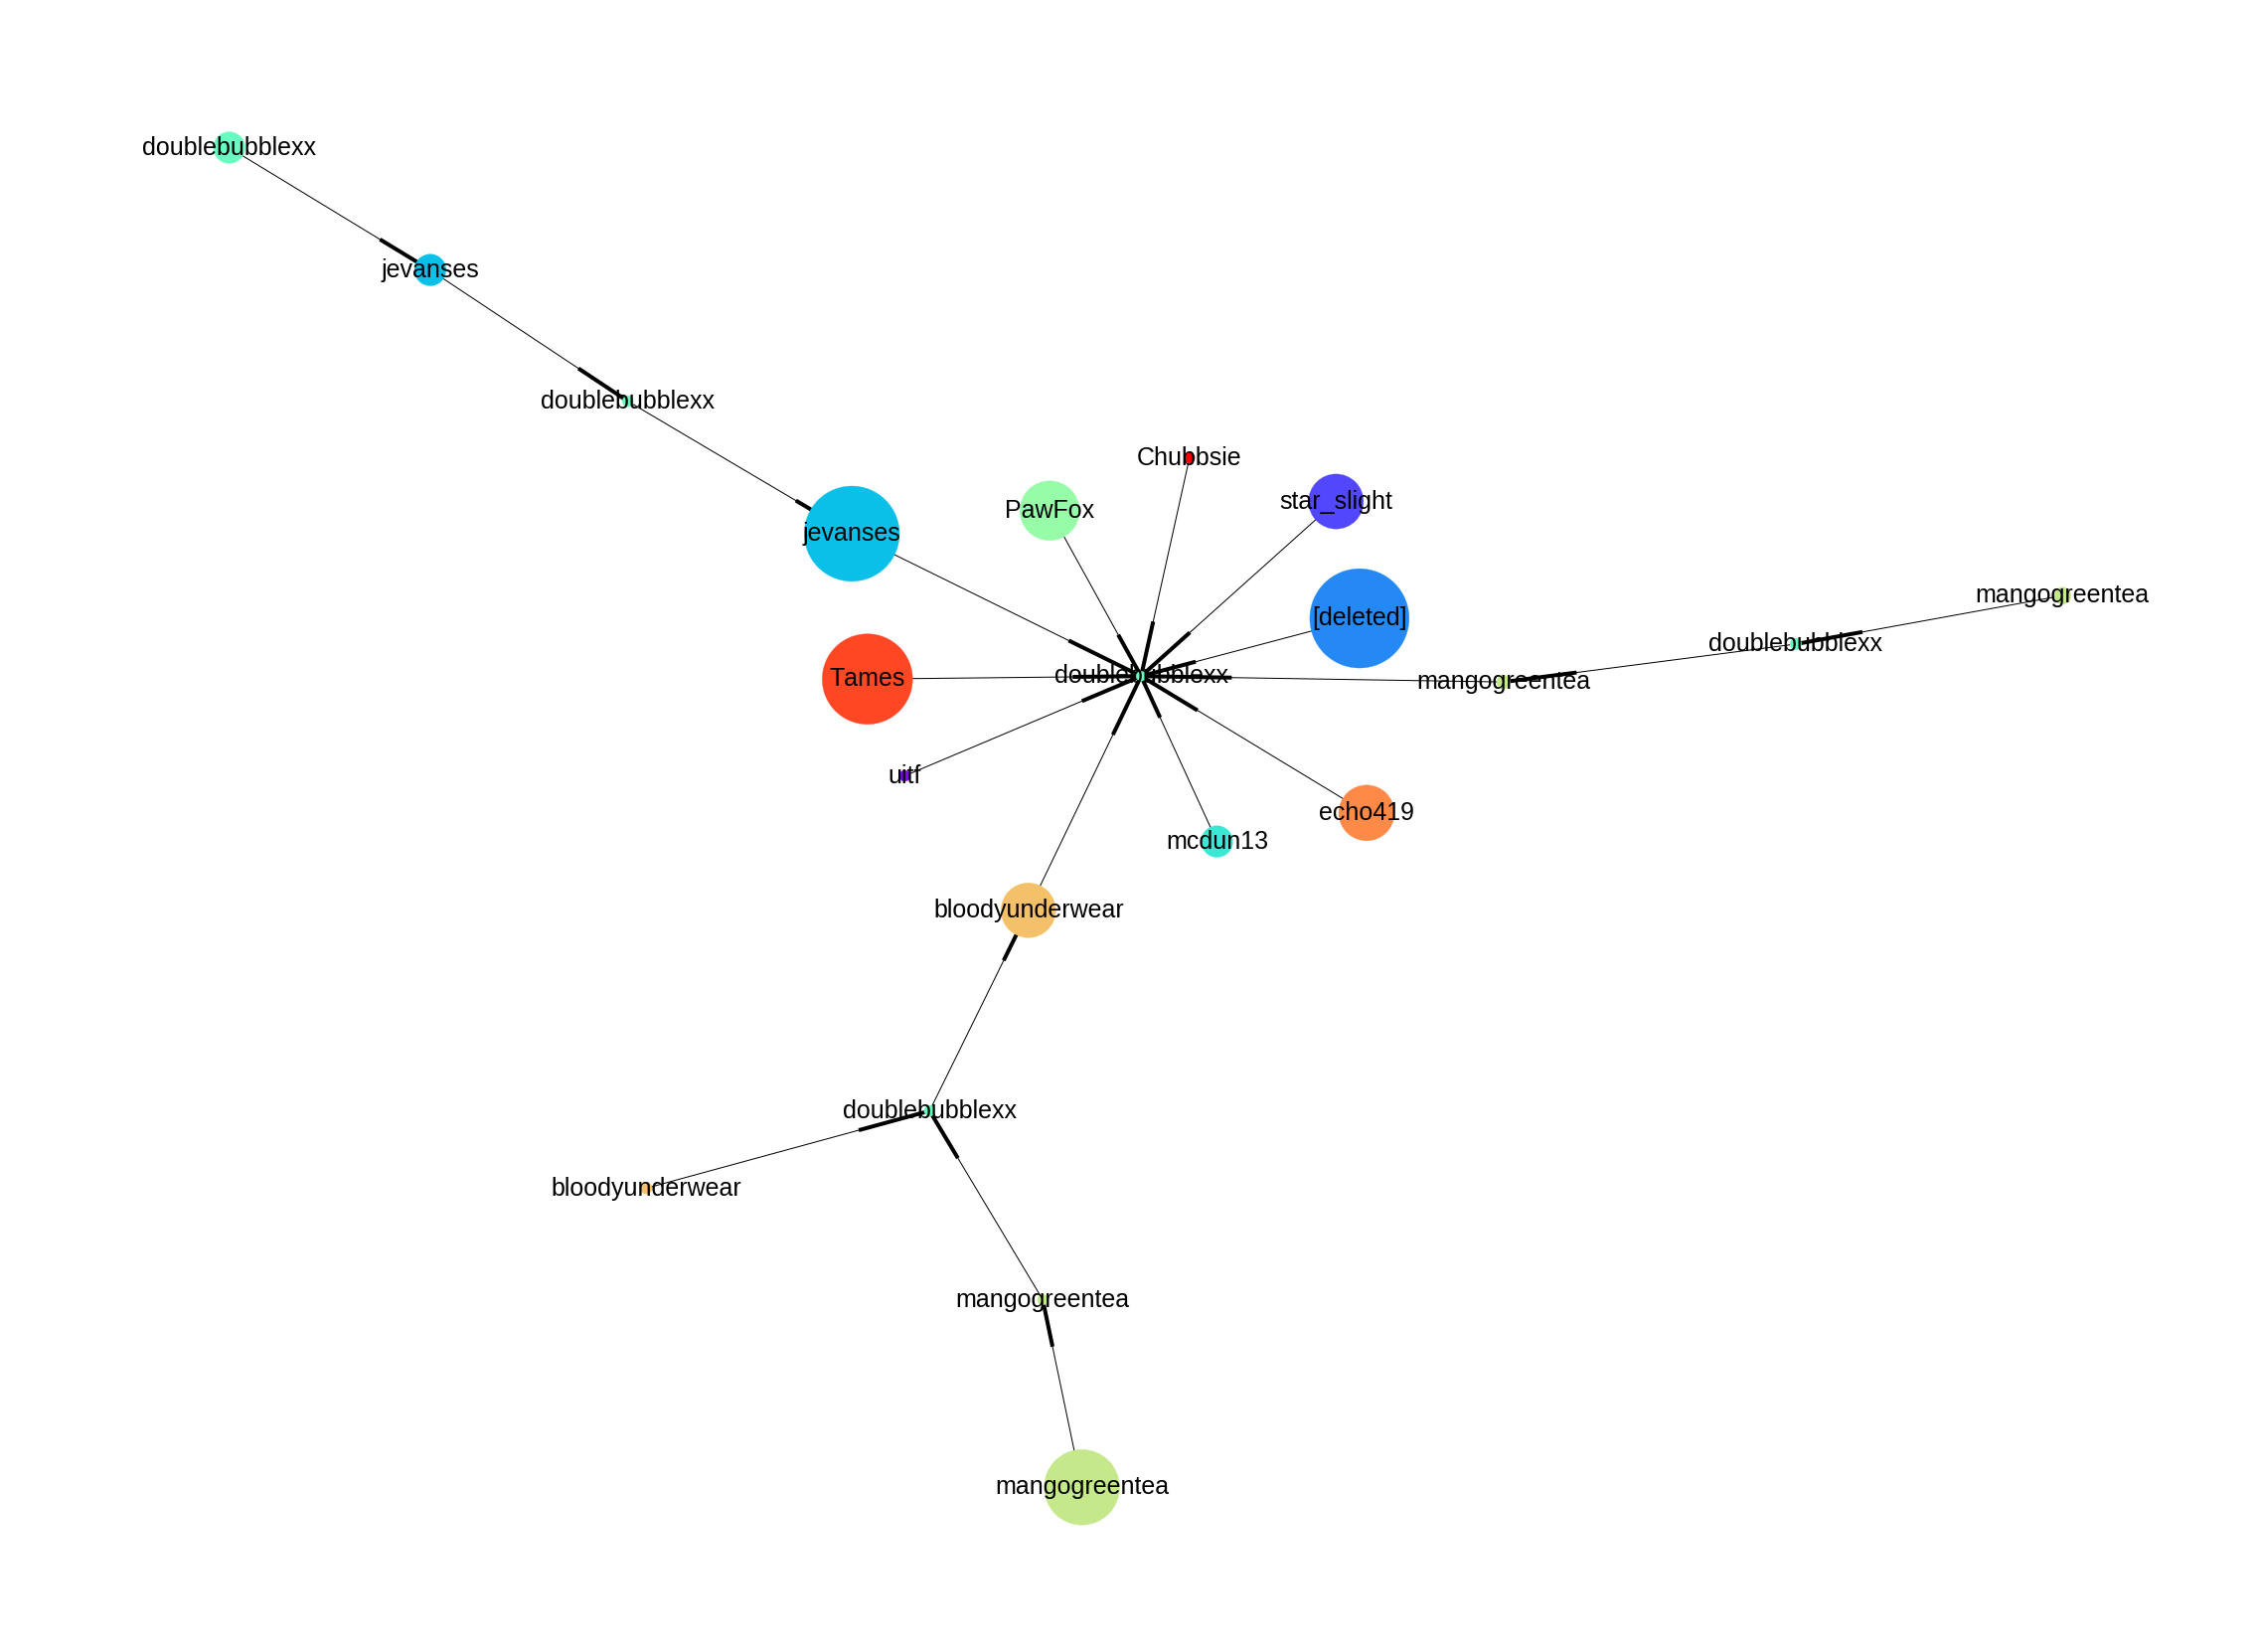
\includegraphics[width=0.45\textwidth, height = 5cm ]{Figures/ReplyGraphSW}
		\label{fig:rGraphSW}
	}
	\subfloat[]{
		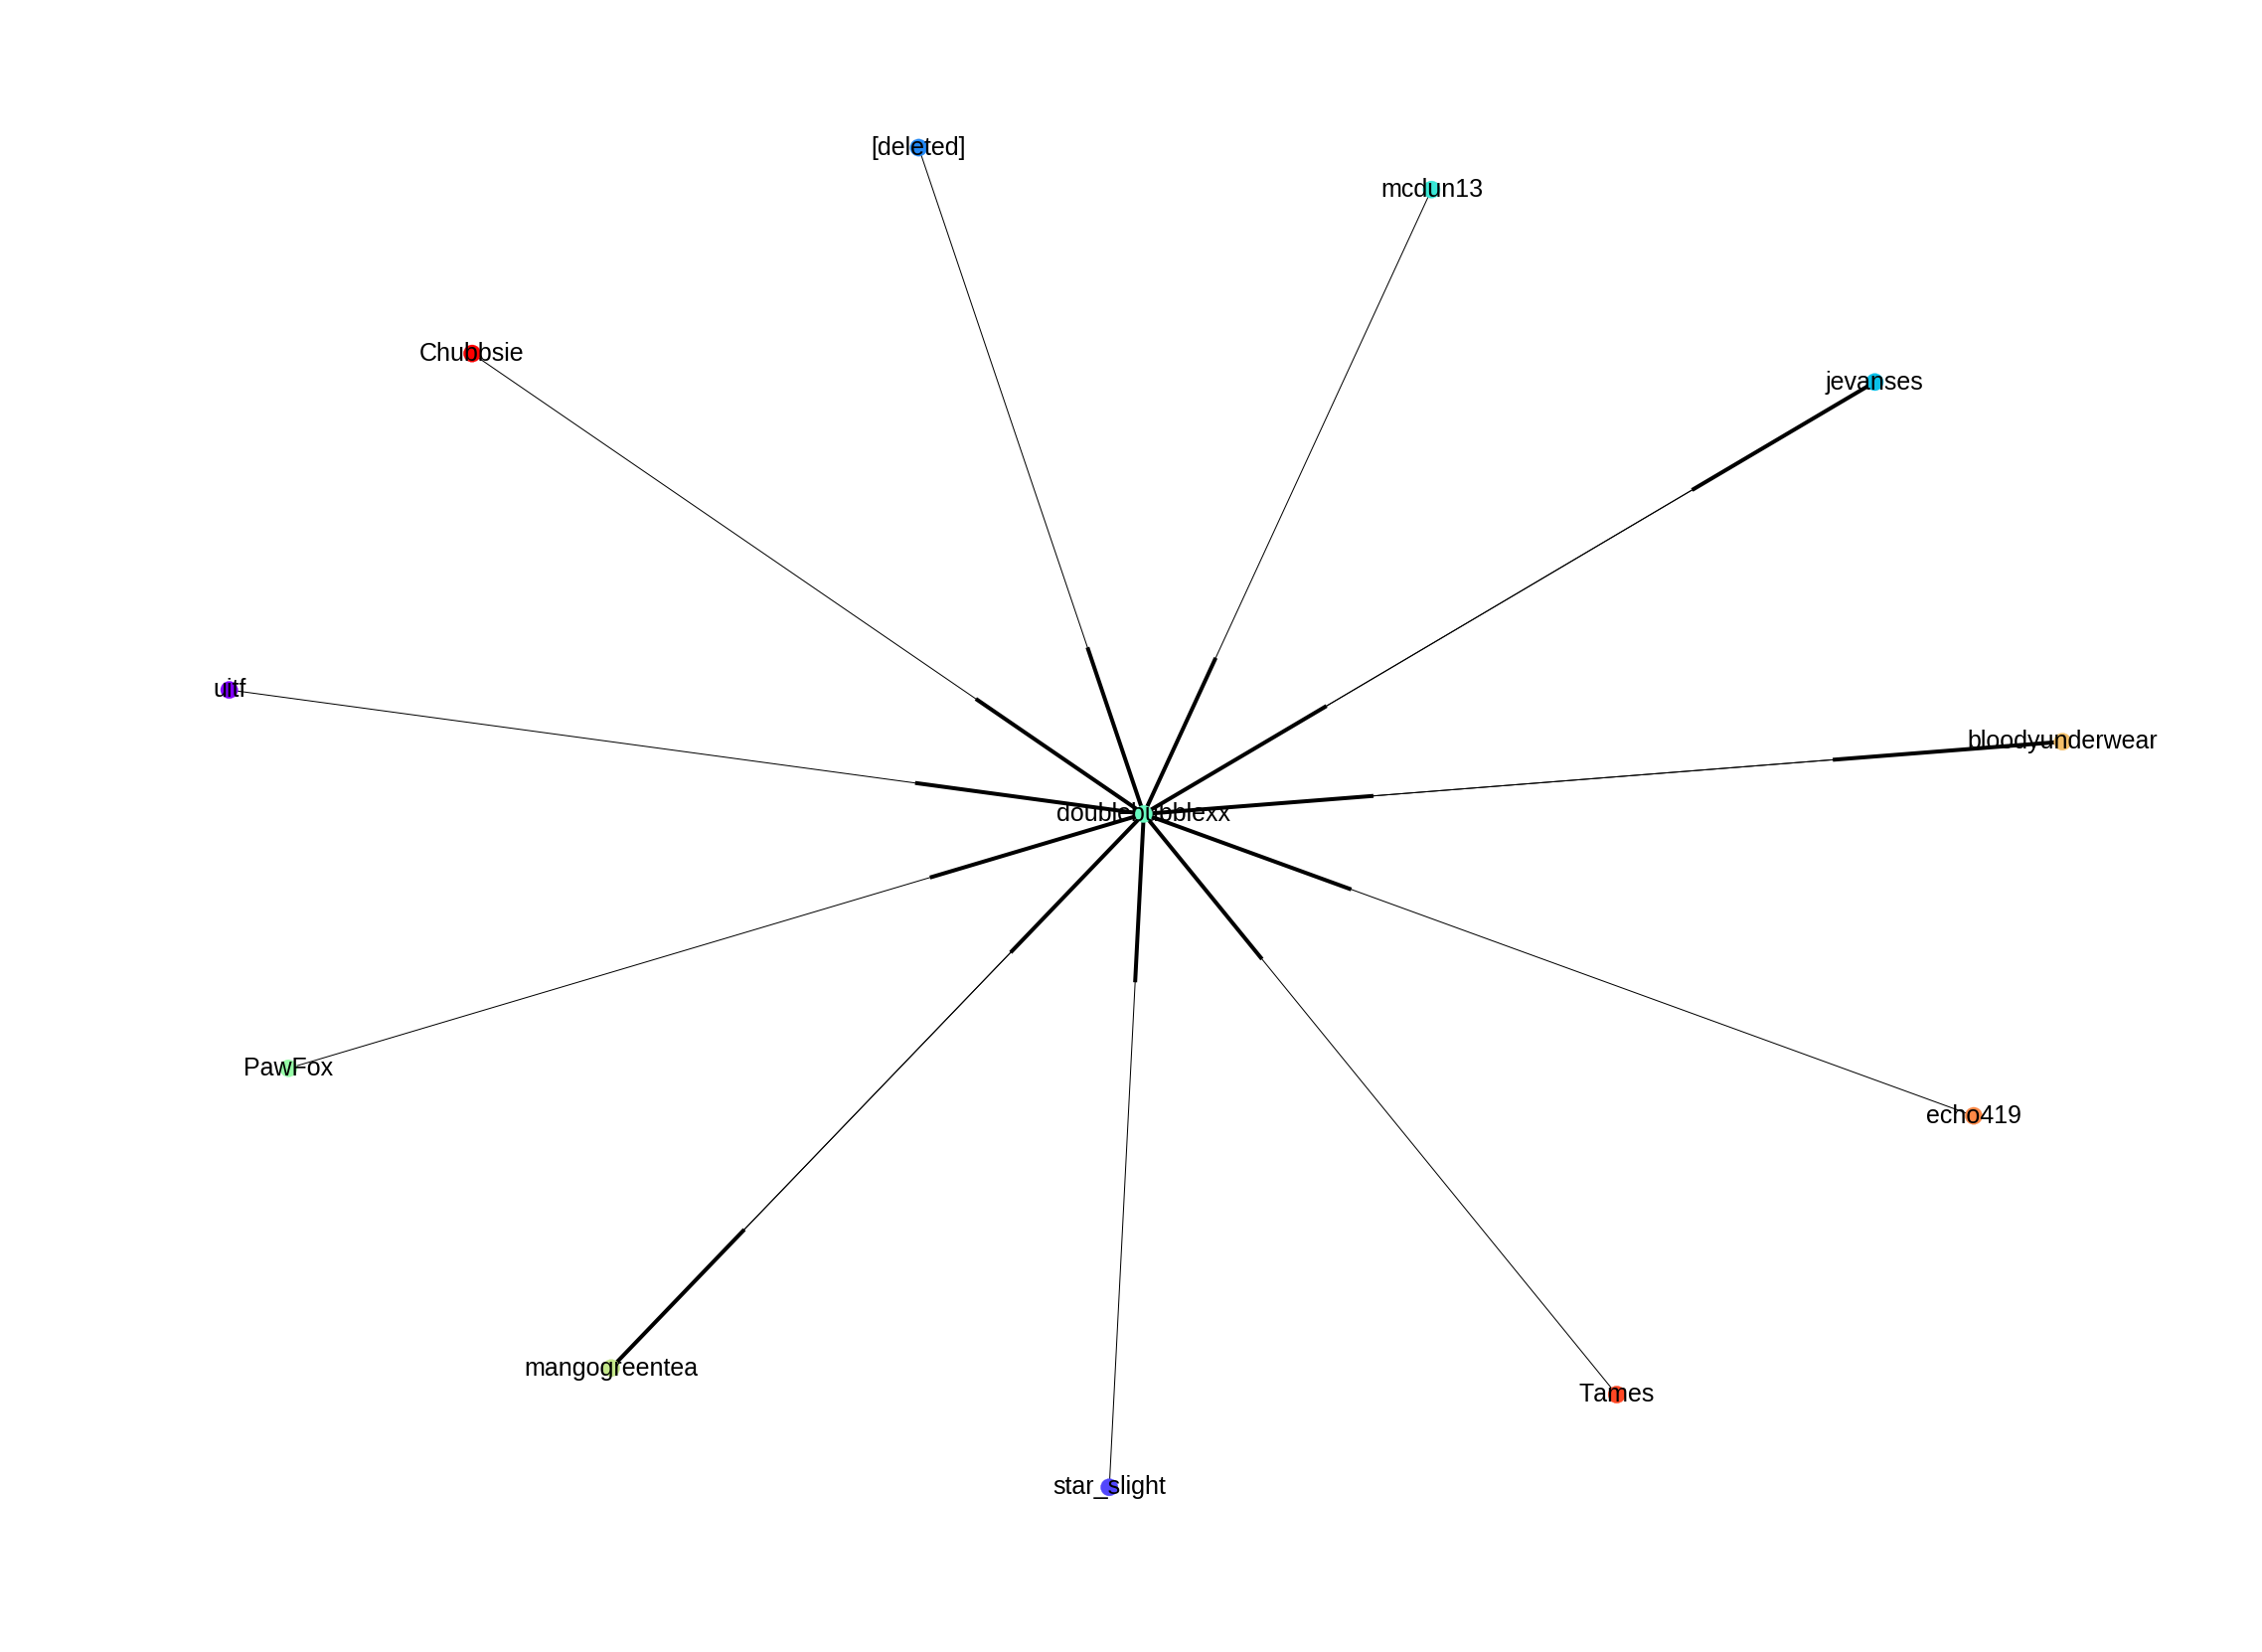
\includegraphics[width=0.45\linewidth, height = 5cm ]{Figures/UserGraphSW}
		\label{fig:uGraphSW}
	}


	\subfloat[]{
		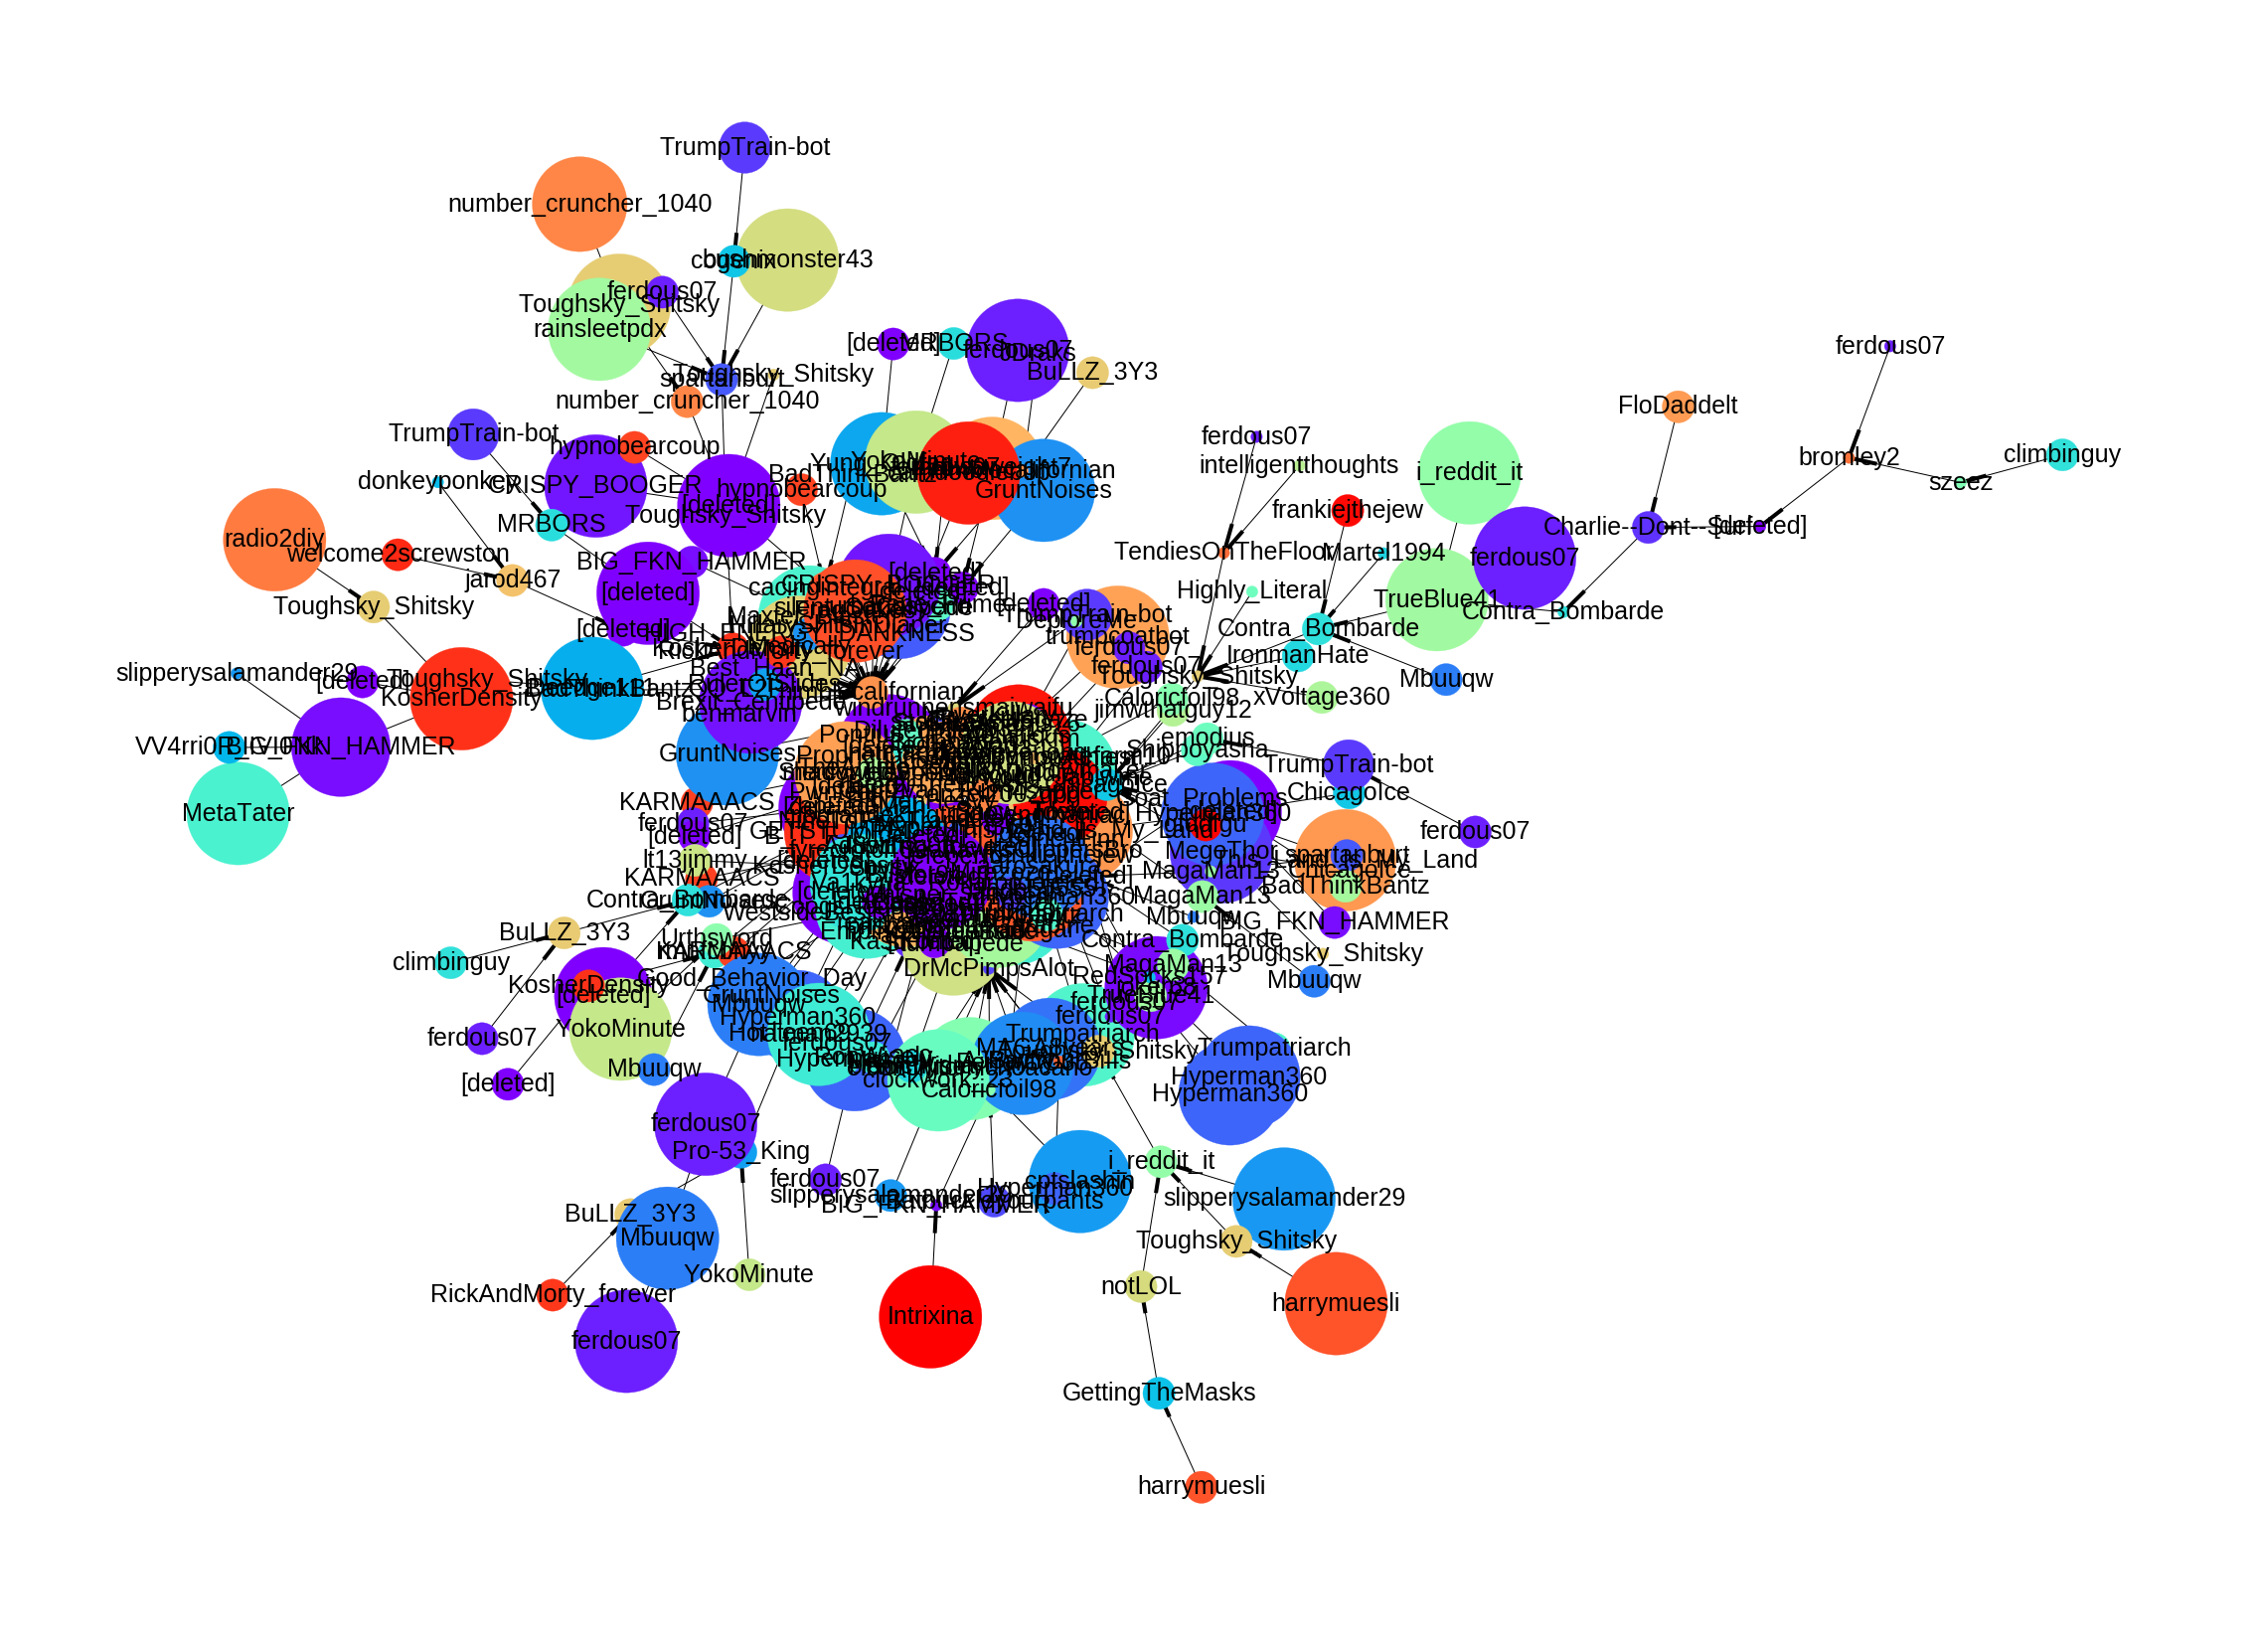
\includegraphics[width=0.45\linewidth, height = 5cm ]{Figures/ReplyGraphTD}
		\label{fig:rGraphTD}
	}
	\subfloat[]{
		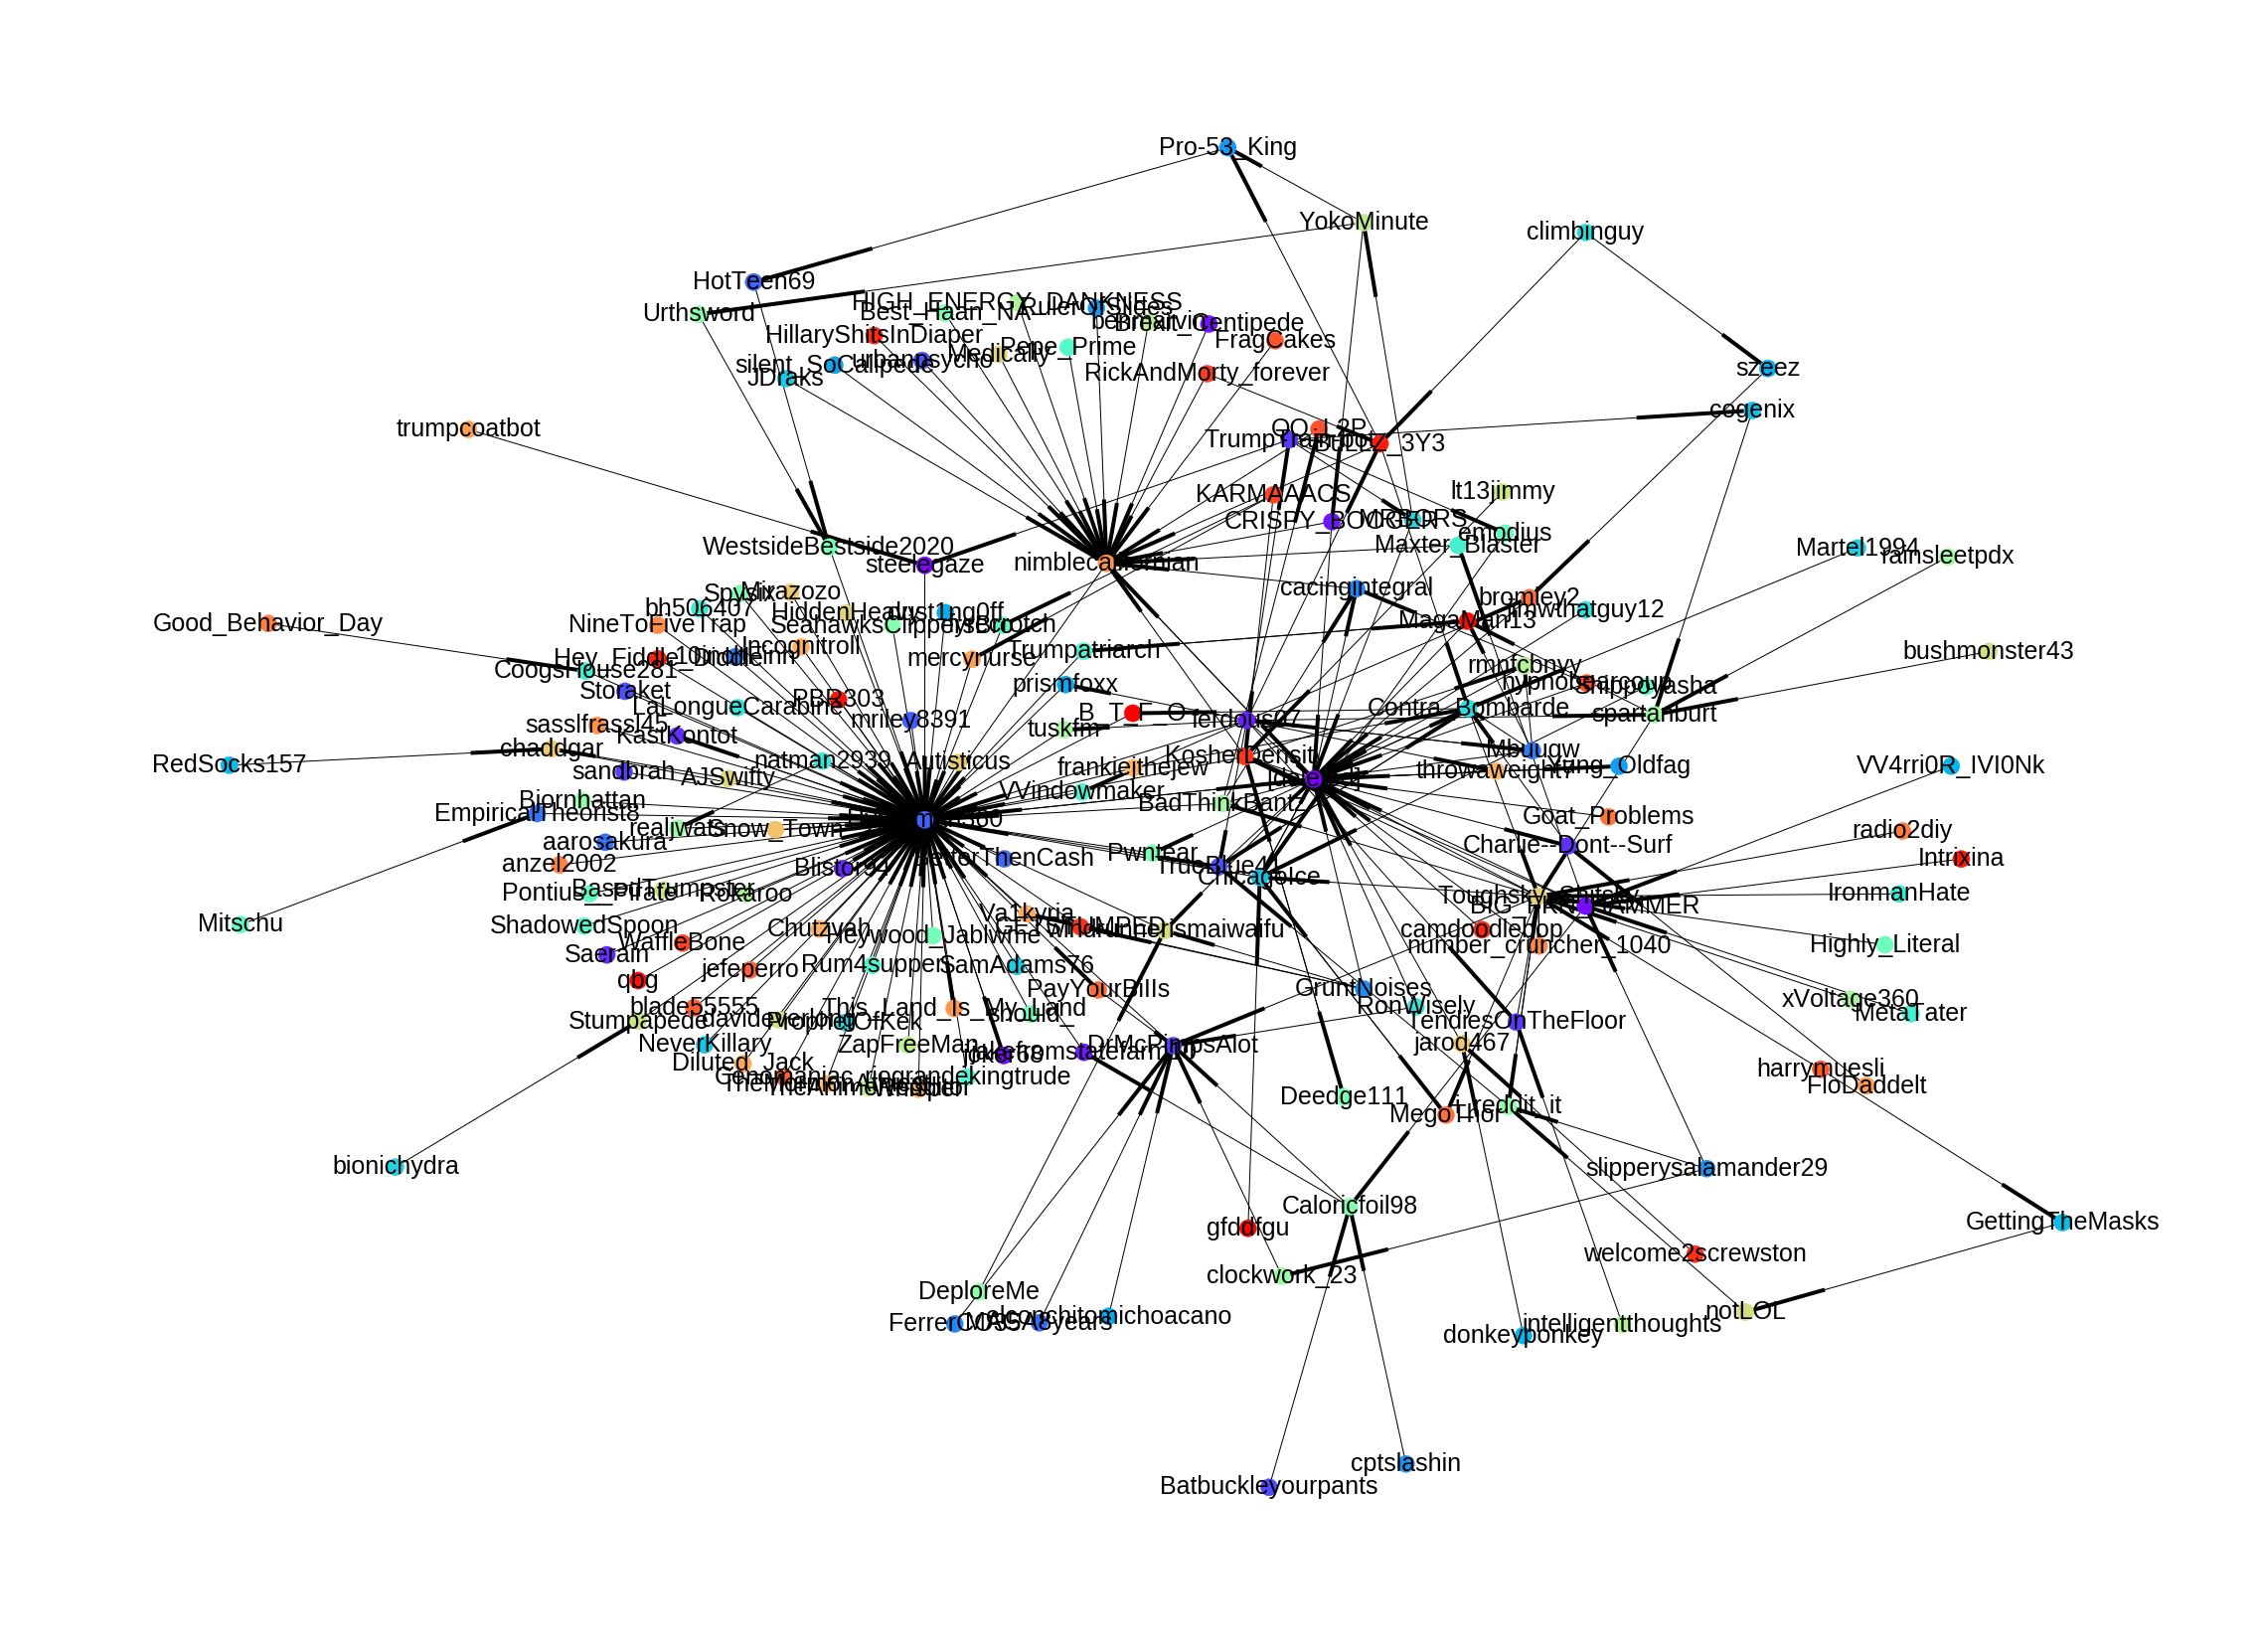
\includegraphics[width=0.45\linewidth, height = 5cm ]{Figures/UserGraphTD}
		\label{fig:uGraphTD}
	}
	\caption{ Example UserGraphs and their corresponding Reply graphs, Figure \ref{fig:uGraphSW} shows a random thread from the SW sub-reddit and \ref{fig:rGraphSW} shows the corresponding reply graph that arises from the response structure of the same thread. In comparison we have Usergraph Fig \ref{fig:uGraphTD} and its corresponding reply graph Fig \ref{fig:rGraphTD} from the subreddit r/TheDonald }
	\label{Fig:GraphExamples}
\end{figure*}


